\documentclass{standalone}
\usepackage{tikz}
\usetikzlibrary{patterns, positioning}
\usepackage[sfdefault]{ClearSans} %% option 'sfdefault' activates Clear Sans as the default text font
\usepackage[T1]{fontenc}

\begin{document}
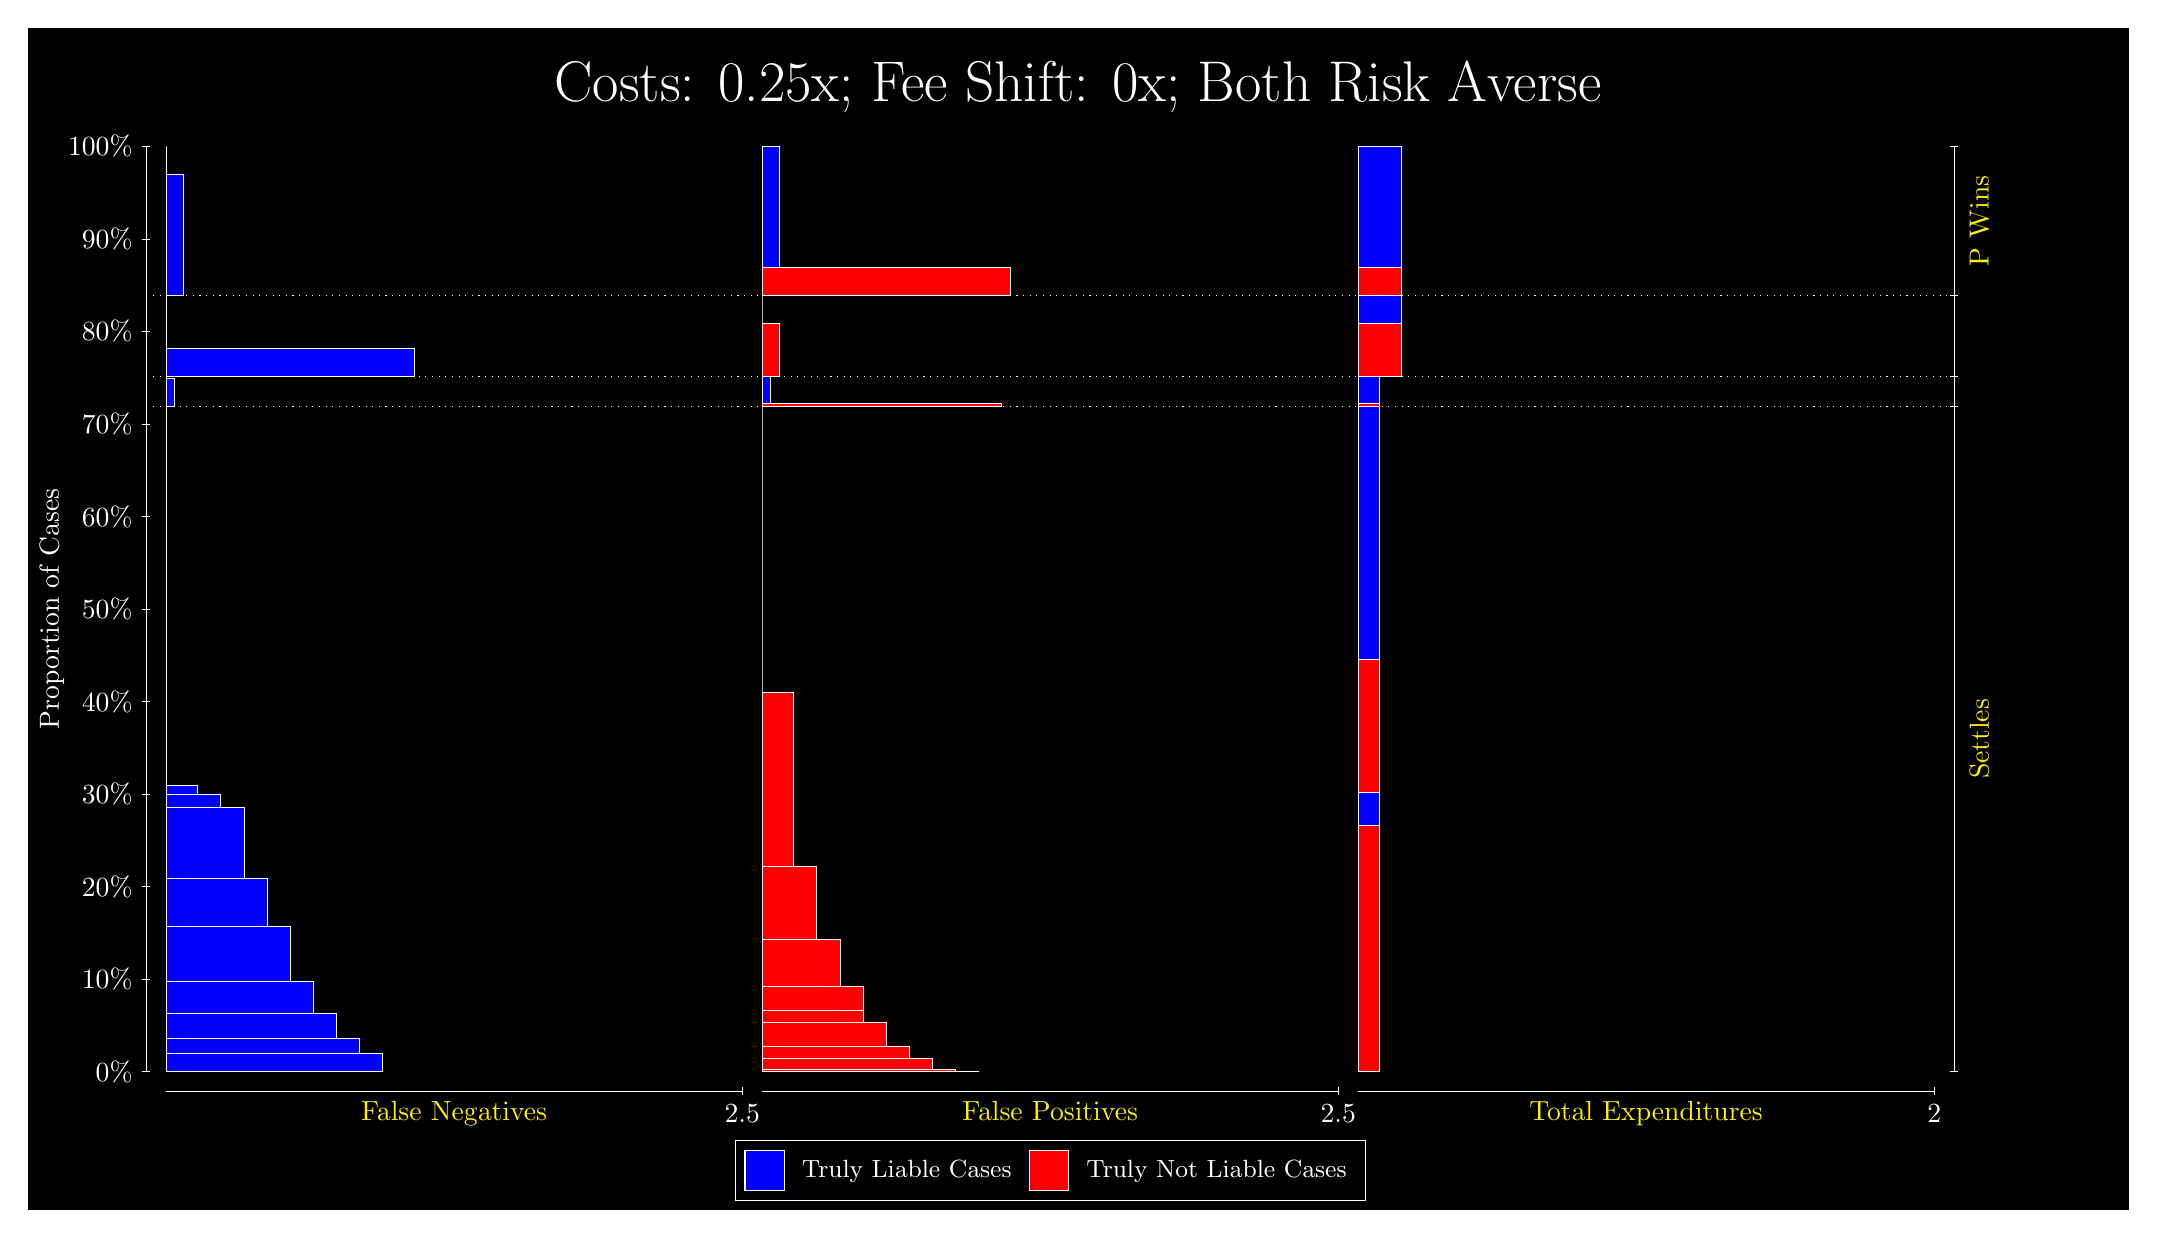
\begin{tikzpicture}
\draw[fill=black] (0,0) rectangle (26.667,15);
\draw[text=white] (0,13.5) rectangle (26.667,15) node[midway] {\huge Costs: 0.25x; Fee Shift: 0x; Both Risk Averse};
\draw[white, very thin] (1.5,1.75) -- (1.5,13.5);
\node[rotate=90, text=white, anchor=center] at (0.3, 7.625) {Proportion of Cases};
\draw[white, very thin] (1.45,1.75) -- (1.55,1.75);
\node[text=white, anchor=east] at (1.45, 1.75) {0\%};
\draw[white, very thin] (1.45,2.925) -- (1.55,2.925);
\node[text=white, anchor=east] at (1.45, 2.925) {10\%};
\draw[white, very thin] (1.45,4.1) -- (1.55,4.1);
\node[text=white, anchor=east] at (1.45, 4.1) {20\%};
\draw[white, very thin] (1.45,5.275) -- (1.55,5.275);
\node[text=white, anchor=east] at (1.45, 5.275) {30\%};
\draw[white, very thin] (1.45,6.45) -- (1.55,6.45);
\node[text=white, anchor=east] at (1.45, 6.45) {40\%};
\draw[white, very thin] (1.45,7.625) -- (1.55,7.625);
\node[text=white, anchor=east] at (1.45, 7.625) {50\%};
\draw[white, very thin] (1.45,8.8) -- (1.55,8.8);
\node[text=white, anchor=east] at (1.45, 8.8) {60\%};
\draw[white, very thin] (1.45,9.975) -- (1.55,9.975);
\node[text=white, anchor=east] at (1.45, 9.975) {70\%};
\draw[white, very thin] (1.45,11.15) -- (1.55,11.15);
\node[text=white, anchor=east] at (1.45, 11.15) {80\%};
\draw[white, very thin] (1.45,12.325) -- (1.55,12.325);
\node[text=white, anchor=east] at (1.45, 12.325) {90\%};
\draw[white, very thin] (1.45,13.5) -- (1.55,13.5);
\node[text=white, anchor=east] at (1.45, 13.5) {100\%};

\draw[white, very thin] (24.457,1.75) -- (24.457,13.5);
\draw[white, very thin] (24.407,1.75) -- (24.507,1.75);
\node[anchor=west] at (24.407, 1.75) {};
\draw[white, very thin] (24.407,10.199) -- (24.507,10.199);
\node[anchor=west] at (24.407, 10.199) {};
\draw[white, very thin] (24.407,10.582) -- (24.507,10.582);
\node[anchor=west] at (24.407, 10.582) {};
\draw[white, very thin] (24.407,11.605) -- (24.507,11.605);
\node[anchor=west] at (24.407, 11.605) {};
\draw[white, very thin] (24.407,13.5) -- (24.507,13.5);
\node[anchor=west] at (24.407, 13.5) {};

\draw[white, very thin, fill=blue] (1.75,1.75) rectangle (4.4946,1.9871);
\draw[white, very thin, fill=blue] (1.75,1.9871) rectangle (4.2018,2.1697);
\draw[white, very thin, fill=blue] (1.75,2.1697) rectangle (3.9091,2.4908);
\draw[white, very thin, fill=blue] (1.75,2.4908) rectangle (3.6163,2.9001);
\draw[white, very thin, fill=blue] (1.75,2.9001) rectangle (3.3236,3.5957);
\draw[white, very thin, fill=blue] (1.75,3.5957) rectangle (3.0308,4.2034);
\draw[white, very thin, fill=blue] (1.75,4.2034) rectangle (2.738,5.1082);
\draw[white, very thin, fill=blue] (1.75,5.1082) rectangle (2.4453,5.2774);
\draw[white, very thin, fill=blue] (1.75,5.2774) rectangle (2.1525,5.3835);
\draw[white, very thin, fill=red] (1.75,5.3835) rectangle (1.75,10.199);
\draw[white, very thin, fill=blue] (1.75,10.199) rectangle (1.8598,10.551);
\draw[white, very thin, fill=red] (1.75,10.551) rectangle (1.75,10.582);
\draw[white, very thin, fill=blue] (1.75,10.582) rectangle (4.8971,10.934);
\draw[white, very thin, fill=red] (1.75,10.934) rectangle (1.75,11.605);
\draw[white, very thin, fill=blue] (1.75,11.605) rectangle (1.9696,13.144);
\draw[white, very thin, fill=red] (1.75,13.144) rectangle (1.75,13.5);
\draw[white, very thin, fill=red] (9.3189,1.75) rectangle (12.063,1.7589);
\draw[white, very thin, fill=red] (9.3189,1.7589) rectangle (11.771,1.7761);
\draw[white, very thin, fill=red] (9.3189,1.7761) rectangle (11.478,1.9197);
\draw[white, very thin, fill=red] (9.3189,1.9197) rectangle (11.185,2.0752);
\draw[white, very thin, fill=red] (9.3189,2.0752) rectangle (10.892,2.3702);
\draw[white, very thin, fill=red] (9.3189,2.3702) rectangle (10.6,2.5228);
\draw[white, very thin, fill=red] (9.3189,2.5228) rectangle (10.6,2.8325);
\draw[white, very thin, fill=red] (9.3189,2.8325) rectangle (10.307,3.435);
\draw[white, very thin, fill=red] (9.3189,3.435) rectangle (10.014,4.3577);
\draw[white, very thin, fill=red] (9.3189,4.3577) rectangle (9.7214,6.5657);
\draw[white, very thin, fill=blue] (9.3189,6.5657) rectangle (9.3189,10.199);
\draw[white, very thin, fill=red] (9.3189,10.199) rectangle (12.356,10.231);
\draw[white, very thin, fill=blue] (9.3189,10.231) rectangle (9.4287,10.582);
\draw[white, very thin, fill=red] (9.3189,10.582) rectangle (9.5384,11.254);
\draw[white, very thin, fill=blue] (9.3189,11.254) rectangle (9.3189,11.605);
\draw[white, very thin, fill=red] (9.3189,11.605) rectangle (12.466,11.962);
\draw[white, very thin, fill=blue] (9.3189,11.962) rectangle (9.5384,13.5);
\draw[white, very thin, fill=red] (16.888,1.75) rectangle (17.162,4.8807);
\draw[white, very thin, fill=blue] (16.888,4.8807) rectangle (17.162,5.3004);
\draw[white, very thin, fill=red] (16.888,5.3004) rectangle (17.162,6.9854);
\draw[white, very thin, fill=blue] (16.888,6.9854) rectangle (17.162,10.199);
\draw[white, very thin, fill=red] (16.888,10.199) rectangle (17.162,10.231);
\draw[white, very thin, fill=blue] (16.888,10.231) rectangle (17.162,10.582);
\draw[white, very thin, fill=red] (16.888,10.582) rectangle (17.437,11.254);
\draw[white, very thin, fill=blue] (16.888,11.254) rectangle (17.437,11.605);
\draw[white, very thin, fill=red] (16.888,11.605) rectangle (17.437,11.962);
\draw[white, very thin, fill=blue] (16.888,11.962) rectangle (17.437,13.5);
\draw[white, dotted] (1.5,10.199) -- (24.457,10.199);
\draw[white, dotted] (1.5,10.582) -- (24.457,10.582);
\draw[white, dotted] (1.5,11.605) -- (24.457,11.605);
\draw[white, very thin] (1.75,1.5) -- (9.0689,1.5);
\node[text=yellow, anchor=north] at (5.4094, 1.5) {False Negatives};
\draw[white, very thin] (9.0689,1.45) -- (9.0689,1.55);
\node[text=white, anchor=north] at (9.0689, 1.45) {2.5};

\draw[white, very thin] (9.3189,1.5) -- (16.638,1.5);
\node[text=yellow, anchor=north] at (12.978, 1.5) {False Positives};
\draw[white, very thin] (16.638,1.45) -- (16.638,1.55);
\node[text=white, anchor=north] at (16.638, 1.45) {2.5};

\draw[white, very thin] (16.888,1.5) -- (24.207,1.5);
\node[text=yellow, anchor=north] at (20.547, 1.5) {Total Expenditures};
\draw[white, very thin] (24.207,1.45) -- (24.207,1.55);
\node[text=white, anchor=north] at (24.207, 1.45) {2};

\node[text=yellow, centered, rotate=90] at (24.777, 5.9746) {Settles};


\node[text=yellow, centered, rotate=90] at (24.777, 12.553) {P Wins};

\draw (12.978300999999998,1.5) node[draw=none] (baseCoordinate) {};
\begin{scope}[align=center]
        \matrix[scale=0.5, draw=white, below=0.5cm of baseCoordinate, nodes={draw}, column sep=0.1cm]{
            \node[rectangle, draw, minimum width=0.5cm, minimum height=0.5cm, fill=blue] {}; &
            \node[draw=none, font=\small, text=white] (B) {Truly Liable Cases}; &
            \node[rectangle, draw, minimum width=0.5cm, minimum height=0.5cm, fill=red] {}; &
            \node[draw=none, font=\small, text=white] (B) {Truly Not Liable Cases}; \\
            };
\end{scope}

\end{tikzpicture}
\end{document}